\section{Comparison Evaluation}
The MH algorithm and VG algorithm are both designed to solve
multidimensional approximate agreement problems. But they use
different methods to get the result. They get different properties
and limitations, and specific application constraints. The HM
algorithm depends on the barycenter of the safe area. The VG
algorithm depends on upper bound and lower bound of the value.

Research proposed that MH algorithm has a faster convergence rate.
From the equations, it is hard to tell. The situations is the
property are different, and it is hard to directly compare both
of the algorithms. 

\subsection{Time complexity}
To compare these algorithms, we choose some value of the setup.
And we use the different dimension as the x-axis to plot the 
number of iterations. The y-axis is the number of iteration.

I choose both $\epsilon$ as 0.5, I assume
$U - v$ as 2, $\gamma$ is 0.5 to plot picture. The dimension is
from 1 to 50. The maximun $\delta_{U}(m)$ is choosed by 1.

% This file was created by matplotlib2tikz v0.6.14.
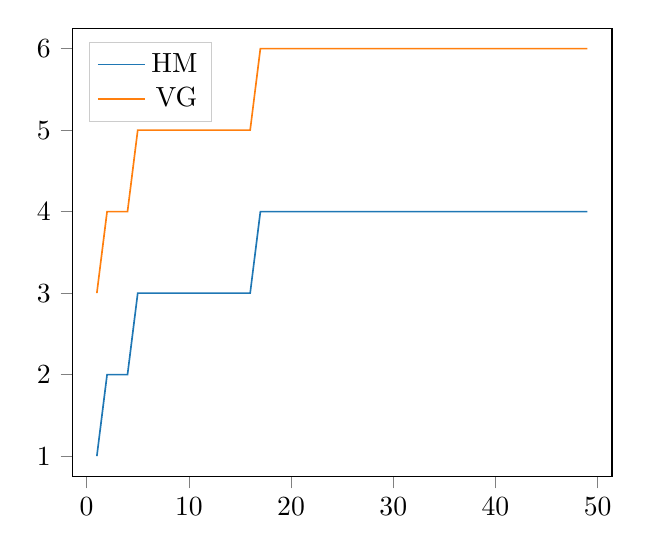
\begin{tikzpicture}

\definecolor{color1}{rgb}{1,0.498039215686275,0.0549019607843137}
\definecolor{color0}{rgb}{0.12156862745098,0.466666666666667,0.705882352941177}

\begin{axis}[
xmin=-1.4, xmax=51.4,
ymin=0.75, ymax=6.25,
tick align=outside,
tick pos=left,
x grid style={lightgray!92.026143790849673!black},
y grid style={lightgray!92.026143790849673!black},
legend style={at={(0.03,0.97)}, anchor=north west, draw=white!80.0!black},
legend cell align={right},
legend entries={{HM},{VG}}
]
\addlegendimage{no markers, color0}
\addlegendimage{no markers, color1}
\addplot [semithick, color0]
table {%
0 -inf
1 1
2 2
3 2
4 2
5 3
6 3
7 3
8 3
9 3
10 3
11 3
12 3
13 3
14 3
15 3
16 3
17 4
18 4
19 4
20 4
21 4
22 4
23 4
24 4
25 4
26 4
27 4
28 4
29 4
30 4
31 4
32 4
33 4
34 4
35 4
36 4
37 4
38 4
39 4
40 4
41 4
42 4
43 4
44 4
45 4
46 4
47 4
48 4
49 4
};
\addplot [semithick, color1]
table {%
0 -inf
1 3
2 4
3 4
4 4
5 5
6 5
7 5
8 5
9 5
10 5
11 5
12 5
13 5
14 5
15 5
16 5
17 6
18 6
19 6
20 6
21 6
22 6
23 6
24 6
25 6
26 6
27 6
28 6
29 6
30 6
31 6
32 6
33 6
34 6
35 6
36 6
37 6
38 6
39 6
40 6
41 6
42 6
43 6
44 6
45 6
46 6
47 6
48 6
49 6
};
\end{axis}

\end{tikzpicture}


From this plot, we can tell that VG algorithm need more iteration
to get converge. And each iteration number is increasing as the 
dimension increasing.

When we choose the a different set of value, the maximun $\delta_{U}(m)$ is choosed by 2.
Using $U - v$ as 4 and plot the number of convergences from
dimension 1 to 50.

% This file was created by matplotlib2tikz v0.6.14.
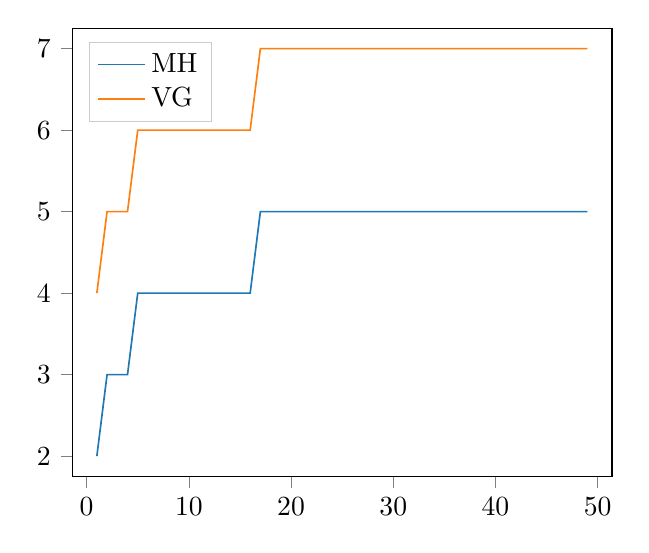
\begin{tikzpicture}

\definecolor{color1}{rgb}{1,0.498039215686275,0.0549019607843137}
\definecolor{color0}{rgb}{0.12156862745098,0.466666666666667,0.705882352941177}

\begin{axis}[
xmin=-1.4, xmax=51.4,
ymin=1.75, ymax=7.25,
tick align=outside,
tick pos=left,
x grid style={lightgray!92.026143790849673!black},
y grid style={lightgray!92.026143790849673!black},
legend entries={{MH},{VG}},
legend cell align={left},
legend style={at={(0.03,0.97)}, anchor=north west, draw=white!80.0!black}
]
\addlegendimage{no markers, color0}
\addlegendimage{no markers, color1}
\addplot [semithick, color0]
table {%
0 -inf
1 2
2 3
3 3
4 3
5 4
6 4
7 4
8 4
9 4
10 4
11 4
12 4
13 4
14 4
15 4
16 4
17 5
18 5
19 5
20 5
21 5
22 5
23 5
24 5
25 5
26 5
27 5
28 5
29 5
30 5
31 5
32 5
33 5
34 5
35 5
36 5
37 5
38 5
39 5
40 5
41 5
42 5
43 5
44 5
45 5
46 5
47 5
48 5
49 5
};
\addplot [semithick, color1]
table {%
0 -inf
1 4
2 5
3 5
4 5
5 6
6 6
7 6
8 6
9 6
10 6
11 6
12 6
13 6
14 6
15 6
16 6
17 7
18 7
19 7
20 7
21 7
22 7
23 7
24 7
25 7
26 7
27 7
28 7
29 7
30 7
31 7
32 7
33 7
34 7
35 7
36 7
37 7
38 7
39 7
40 7
41 7
42 7
43 7
44 7
45 7
46 7
47 7
48 7
49 7
};
\end{axis}

\end{tikzpicture}

From this plot we can tell that these two figure is similar, so we 
want to reduce the value of $\gamma$ to 0.1. The plot is following.

% This file was created by matplotlib2tikz v0.6.14.
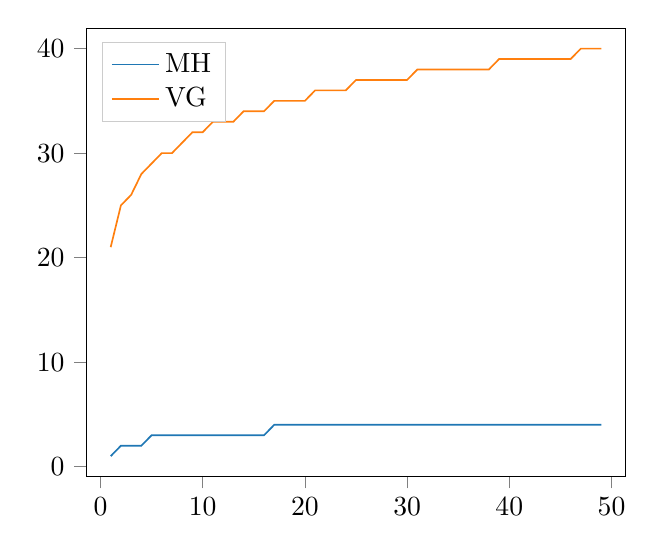
\begin{tikzpicture}

\definecolor{color1}{rgb}{1,0.498039215686275,0.0549019607843137}
\definecolor{color0}{rgb}{0.12156862745098,0.466666666666667,0.705882352941177}

\begin{axis}[
xmin=-1.4, xmax=51.4,
ymin=-0.95, ymax=41.95,
tick align=outside,
tick pos=left,
x grid style={lightgray!92.026143790849673!black},
y grid style={lightgray!92.026143790849673!black},
legend entries={{MH},{VG}},
legend cell align={left},
legend style={at={(0.03,0.97)}, anchor=north west, draw=white!80.0!black}
]
\addlegendimage{no markers, color0}
\addlegendimage{no markers, color1}
\addplot [semithick, color0]
table {%
0 -inf
1 1
2 2
3 2
4 2
5 3
6 3
7 3
8 3
9 3
10 3
11 3
12 3
13 3
14 3
15 3
16 3
17 4
18 4
19 4
20 4
21 4
22 4
23 4
24 4
25 4
26 4
27 4
28 4
29 4
30 4
31 4
32 4
33 4
34 4
35 4
36 4
37 4
38 4
39 4
40 4
41 4
42 4
43 4
44 4
45 4
46 4
47 4
48 4
49 4
};
\addplot [semithick, color1]
table {%
0 -inf
1 21
2 25
3 26
4 28
5 29
6 30
7 30
8 31
9 32
10 32
11 33
12 33
13 33
14 34
15 34
16 34
17 35
18 35
19 35
20 35
21 36
22 36
23 36
24 36
25 37
26 37
27 37
28 37
29 37
30 37
31 38
32 38
33 38
34 38
35 38
36 38
37 38
38 38
39 39
40 39
41 39
42 39
43 39
44 39
45 39
46 39
47 40
48 40
49 40
};
\end{axis}

\end{tikzpicture}

From this plot we can tell that when $\gamma$ goes to 0, the iteration
of VG algorithm will decrease dramaticlly.

% This file was created by matplotlib2tikz v0.6.14.
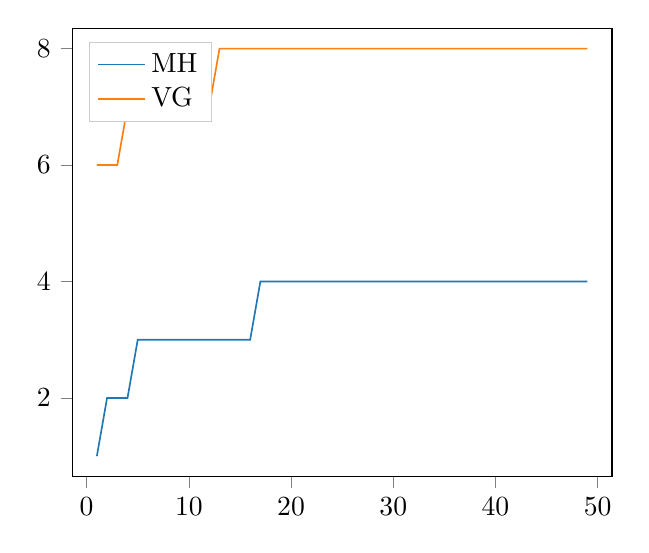
\begin{tikzpicture}

\definecolor{color1}{rgb}{1,0.498039215686275,0.0549019607843137}
\definecolor{color0}{rgb}{0.12156862745098,0.466666666666667,0.705882352941177}

\begin{axis}[
xmin=-1.4, xmax=51.4,
ymin=0.65, ymax=8.35,
tick align=outside,
tick pos=left,
x grid style={lightgray!92.026143790849673!black},
y grid style={lightgray!92.026143790849673!black},
legend entries={{MH},{VG}},
legend cell align={left},
legend style={at={(0.03,0.97)}, anchor=north west, draw=white!80.0!black}
]
\addlegendimage{no markers, color0}
\addlegendimage{no markers, color1}
\addplot [semithick, color0]
table {%
0 -inf
1 1
2 2
3 2
4 2
5 3
6 3
7 3
8 3
9 3
10 3
11 3
12 3
13 3
14 3
15 3
16 3
17 4
18 4
19 4
20 4
21 4
22 4
23 4
24 4
25 4
26 4
27 4
28 4
29 4
30 4
31 4
32 4
33 4
34 4
35 4
36 4
37 4
38 4
39 4
40 4
41 4
42 4
43 4
44 4
45 4
46 4
47 4
48 4
49 4
};
\addplot [semithick, color1]
table {%
0 -inf
1 6
2 6
3 6
4 7
5 7
6 7
7 7
8 7
9 7
10 7
11 7
12 7
13 8
14 8
15 8
16 8
17 8
18 8
19 8
20 8
21 8
22 8
23 8
24 8
25 8
26 8
27 8
28 8
29 8
30 8
31 8
32 8
33 8
34 8
35 8
36 8
37 8
38 8
39 8
40 8
41 8
42 8
43 8
44 8
45 8
46 8
47 8
48 8
49 8
};
\end{axis}

\end{tikzpicture}

From this plot we can see that when $U - v$ is growing, the iteration
time will keep increasing. 

\subsection{Running Time}
